\documentclass[landscape,final,paperwidth=72in,paperheight=42in,fontscale=0.285]{baposter}
%\usepackage{calc,array} 
\usepackage{graphicx} % Required for including images
\usepackage{amsmath}  % For typesetting math
\usepackage{amssymb}  % Adds new symbols to be used in math mode
\usepackage{relsize}  % Chagnge size of text /smaller, /larger
\usepackage{multirow} % Allows table cells to span more than one row of the table
\usepackage{rotating} % Rotate figures and tables
\usepackage{bm}       % Allows a math expression to be bold
\usepackage{url}      % Allows email address and websites
\usepackage{gensymb}  % Allows degree symbol

\usepackage{float}
\usepackage{caption} % Required for specifying captions to tables and figures
\usepackage[export]{adjustbox}

\captionsetup[figure]{font=Large,skip=0pt,labelformat=empty,justification=raggedright,singlelinecheck=false}

\usepackage{multicol} % Required for multiple columns

\usepackage[utf8]{inputenc} %Required for IEEE reference style
\newcommand{\BIBdecl}{\setlength{\itemsep}{-0.25 em}} %Removes line space between references

% Fonts
%\usepackage{times}
%\usepackage{helvet}
%\usepackage{bookman}
\usepackage{palatino}

%\newcommand{\captionfont}{\footnotesize}

\graphicspath{{images/}{../images/}}
%\usetikzlibrary{calc}

\newcommand{\SET}[1]  {\ensuremath{\mathcal{#1}}}
\newcommand{\MAT}[1]  {\ensuremath{\boldsymbol{#1}}}
\newcommand{\VEC}[1]  {\ensuremath{\boldsymbol{#1}}}
\newcommand{\Video}{\SET{V}}
\newcommand{\video}{\VEC{f}}
\newcommand{\track}{x}
\newcommand{\Track}{\SET T}
\newcommand{\LMs}{\SET L}
\newcommand{\lm}{l}
\newcommand{\PosE}{\SET P}
\newcommand{\posE}{\VEC p}
\newcommand{\negE}{\VEC n}
\newcommand{\NegE}{\SET N}
\newcommand{\Occluded}{\SET O}
\newcommand{\occluded}{o}

%%%%%%%%%%%%%%%%%%%%%%%%%%%%%%%%%%%%%%%%%%%%%%%%%%%%%%%%%%%%%%%%%%%%%%%%%%%%%%%%
% Multicol Settings
%%%%%%%%%%%%%%%%%%%%%%%%%%%%%%%%%%%%%%%%%%%%%%%%%%%%%%%%%%%%%%%%%%%%%%%%%%%%%%%%
\setlength{\columnsep}{1.5em}
\setlength{\columnseprule}{0mm}
%%%%%%%%%%%%%%%%%%%%%%%%%%%%%%%%%%%%%%%%%%%%%%%%%%%%%%%%%%%%%%%%%%%%%%%%%%%%%%%%
% Save space in lists. Use this after the opening of the list
%%%%%%%%%%%%%%%%%%%%%%%%%%%%%%%%%%%%%%%%%%%%%%%%%%%%%%%%%%%%%%%%%%%%%%%%%%%%%%%%
\newcommand{\compresslist}{%
\setlength{\itemsep}{1pt}%
\setlength{\parskip}{0pt}%
\setlength{\parsep}{0pt}%
}
%%%%%%%%%%%%%%%%%%%%%%%%%%%%%%%%%%%%%%%%%%%%%%%%%%%%%%%%%%%%%%%%%%%%%%%%%%%%%%
%%% Begin of Document
%%%%%%%%%%%%%%%%%%%%%%%%%%%%%%%%%%%%%%%%%%%%%%%%%%%%%%%%%%%%%%%%%%%%%%%%%%%%%%

\begin{document}

%%%%%%%%%%%%%%%%%%%%%%%%%%%%%%%%%%%%%%%%%%%%%%%%%%%%%%%%%%%%%%%%%%%%%%%%%%%%%%
%%% Here starts the poster
%%%---------------------------------------------------------------------------
%%% Format it to your taste with the options
%%%%%%%%%%%%%%%%%%%%%%%%%%%%%%%%%%%%%%%%%%%%%%%%%%%%%%%%%%%%%%%%%%%%%%%%%%%%%%
% Define some colors

%\definecolor{lightblue}{cmyk}{0.83,0.24,0,0.12}
\definecolor{lightblue}{rgb}{0.145,0.6666,1}

%\newtcolorbox{demobox}[1][]{colback=white,colframe=lightblue,width=0.33\linewidth,nobeforeafter,box align=top,before=\noindent,#1}

%%
\begin{poster}%
  % Poster Options
  {
  % Show grid to help with alignment
  grid=false,
  % Column spacing
  colspacing=1em,
  % Color style
  bgColorOne=white,
  bgColorTwo=white,
  borderColor=lightblue,
  headerColorOne=black,
  headerColorTwo=lightblue,
  headerFontColor=white,
  boxColorOne=white,
  boxColorTwo=lightblue,
  % Format of textbox
  textborder=roundedleft,
  % Format of text header
  eyecatcher=true,
  headerborder=closed,
  headerheight=0.12\textheight,
  columns=5, %default=4 for landscape posters maximum columns=6
%  textfont=\sc, An example of changing the text font
  headershape=roundedright,
  headershade=shadelr,
  headerfont=\Large\bf\textsc, %Sans Serif
  textfont={\setlength{\parindent}{1.5em}},
  boxshade=plain,
%  background=shade-tb,
  background=plain,
  linewidth=2pt
  }
  % University logo
  {
\includegraphics[height=6em]{img/penn_state_cla_logo_new_210-89.jpg}}
  % Title
  {\bf{The appearance and disappearance of visual forms defined by differential motion \\ evokes distinctive EEG responses in school-age children} \vspace{0.2em}}
  % Authors
  {Rick O. Gilmore \emph{(rogilmore@psu.edu)}, Daved A. Fared, Michael G. Dexheimer, \& Andrea R. Seisler\\ \vspace{0.2em}
  Neuroscience 2016 -- Poster 4367}
  % Databrary Logo
 {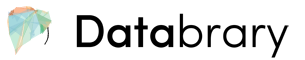
\includegraphics[height=4em]{img/databrary.png}}

%%%%%%%%%%%%%%%%%%%%%%%%%%%%%%%%%%%%%%%%%%%%%%%%%%%%%%%%%%%%%%%%%%%%%%%%%%%%%%
%%% Now define the boxes that make up the poster
%%%---------------------------------------------------------------------------
%%% Each box has a name and can be placed absolutely or relatively.
%%% The only inconvenience is that you can only specify a relative position
%%% towards an already declared box. So if you have a box attached to the
%%% bottom, one to the top and a third one which should be in between, you
%%% have to specify the top and bottom boxes before you specify the middle
%%% box.
%%%%%%%%%%%%%%%%%%%%%%%%%%%%%%%%%%%%%%%%%%%%%%%%%%%%%%%%%%%%
%
%%%%%%%%%%%%%%%%%%%%%%%%%%%%%%%%%%%%%%%%%%%%%%%%%%%%%%%%%%%%%%%%%%%%%%%%%%%%%%
\headerbox{Motivation}{name=abstract,column=0,span = 2,row=0}
%%%%%%%%%%%%%%%%%%%%%%%%%%%%%%%%%%%%%%%%%%%%%%%%%%%%%%%%%%%%%%%%%%%%%%%%%%%%%%
    {
      Differential motion patterns aid in the segmentation of visual figures from the background. 
      Adults show evoked brain responses to time-varying motion-defined forms over posterior scalp regions \cite{fesi_cortical_2014},\cite{fesi_distinct_2011}; in these participants, EEG amplitudes scale with the magnitude of direction differences between the figure and background.
      Little is known about the development of brain responses to motion-defined forms in childhood \cite{gilmore_childrens_2016}. In this study, we measured steady-state visual evoked potential (SSVEP) responses in school-age participants and compared the resulting patterns to previous results of adults.    
    }
%%%%%%%%%%%%%%%%%%%%%%%%%%%%%%%%%%%%%%%%%%%%%%%%%%%%%%%%%%%%%%%%%%%%%%%%%%%%%%
\headerbox{Method}{name=method,column=0,span = 2,below=abstract}
%%%%%%%%%%%%%%%%%%%%%%%%%%%%%%%%%%%%%%%%%%%%%%%%%%%%%%%%%%%%%%%%%%%%%%%%%%%%%%
    {
      School-age observers (n=37; 4.3-9.0 years, \emph{M}=6.4, 16 female) participated in this study.  
      Participants passively viewed random dot kinematogram displays that depicted visual forms which differed in direction from uniform background motion by 5\degree, 45\degree, or 180\degree. Four 9x9 deg square-shaped figure regions emerged from and disappeared into the background at a rate of 1.2 Hz (F1). Figure and background regions were populated with white (39 cd/m\textsuperscript{2}) dots on a black (.065 cd/m\textsuperscript{2}) background at a density of 10\%; dot positions were updated at 36 Hz (F2). Each condition was presented at two speeds (1.2 and 6.0 deg/s). All patterns were displayed in an annular region 24\degree in outer and 4.8\degree inner diameter at the 60 cm viewing distance.  
      EEG was collected at 432.43 Hz using a 128 channel EGI system and PowerDiva Video 3.4 software and submitted to a discrete Fourier transform. 
      The complex domain (real and imaginary) components of each channel were analyzed using mixed-effects MANOVA, with direction difference and speed as fixed factors and participant as a random factor.  
      }
%%%%%%%%%%%%%%%%%%%%%%%%%%%%%%%%%%%%%%%%%%%%%%%%%%%%%%%%%%%%%%%%%%%%%%%%%%%%%%
\headerbox{Displays}{name=displays,column=0, span=2, below=method, above=bottom}
%%%%%%%%%%%%%%%%%%%%%%%%%%%%%%%%%%%%%%%%%%%%%%%%%%%%%%%%%%%%%%%%%%%%%%%%%%%%%%
    {
\begin{figure}[H]
  \centering
  \caption{Laminar}\label{moco-inf-2pat-lamrad-laminar.jpg}
  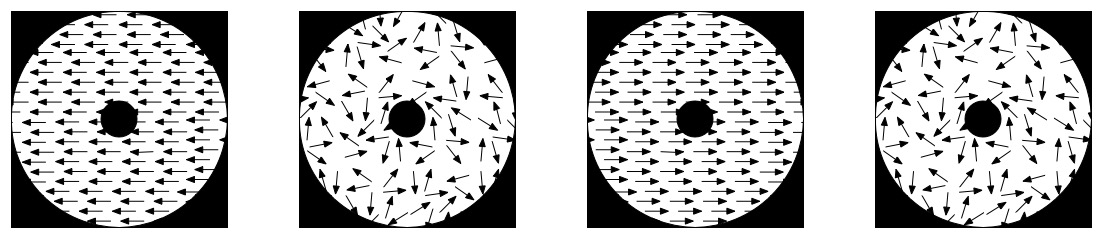
\includegraphics[scale=0.51]{img/moco-inf-2pat-lamrad-laminar.jpg}
  \vspace{0.5em}

  \caption{Radial}\label{moco-inf-2pat-lamrad-radial.jpg}
  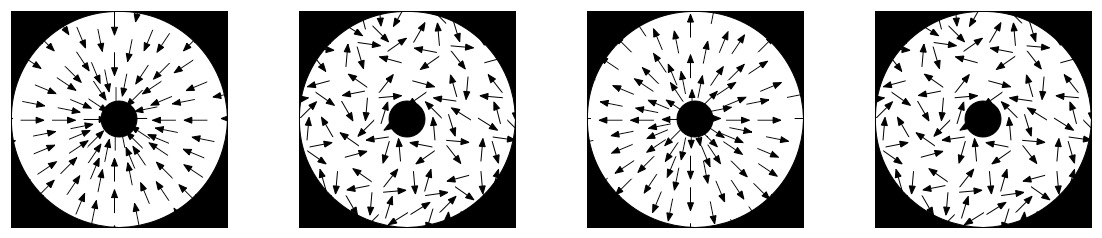
\includegraphics[scale=0.51]{moco-inf-2pat-lamrad-radial.jpg}
  \vspace{0.5em}
    }
%%%%%%%%%%%%%%%%%%%%%%%%%%%%%%%%%%%%%%%%%%%%%%%%%%%%%%%%%%%%%%%%%%%%%%%%%%%%%%
\headerbox{Results - 1F1}{name=1F1,column=2,span=3,row=0}
%%%%%%%%%%%%%%%%%%%%%%%%%%%%%%%%%%%%%%%%%%%%%%%%%%%%%%%%%%%%%%%%%%%%%%%%%%%%%%
%      We chose p<.0005 as our alpha level to reduce the likelihood of reporting false positives. 
%Statistically significant effects for direction were found at 1F1, 2F1, and 3F1, and these showed a broad distribution across the scalp. 
%No channels met criterion for the effect of speed at any harmonic. 
%Many, but not all channels showed the scaling of amplitude by figure/background direction difference found in adults, an effect particularly pronounced at 3F1. 
%Complex domain plots of the most reponsive channels at 2F1 and 3F1 showed consistent phase and amplitude profiles. 
{

\begin{center}

  \includegraphics[scale=0.25,valign=t]{img/1F1-analyze-and-plot-main-effects-1.png}
  \hfill
  \includegraphics[scale=0.18,valign=t]{img/1F1-plot-channel-effects-1.png}
  \hfill
  \includegraphics[scale=0.18,valign=t]{img/1F1-plot-vector-avg-1.png}
  
\end{center}

}
%%%%%%%%%%%%%%%%%%%%%%%%%%%%%%%%%%%%%%%%%%%%%%%%%%%%%%%%%%%%%%%%%%%%%%%%%%%%%%
\headerbox{Results - 2F1}{name=2F1,column=2,span=3,below=1F1}
%%%%%%%%%%%%%%%%%%%%%%%%%%%%%%%%%%%%%%%%%%%%%%%%%%%%%%%%%%%%%%%%%%%%%%%%%%%%%%
{

\begin{center}

  \includegraphics[scale=0.25,valign=t]{img/2F1-analyze-and-plot-main-effects-1.png}
  \hfill
  \includegraphics[scale=0.18,valign=t]{img/2F1-plot-channel-effects-1.png}
  \hfill
  \includegraphics[scale=0.18,valign=t]{img/2F1-plot-vector-avg-1.png}
  
\end{center}

}
%%%%%%%%%%%%%%%%%%%%%%%%%%%%%%%%%%%%%%%%%%%%%%%%%%%%%%%%%%%%%%%%%%%%%%%%%%%%%%
\headerbox{Results - 3F1}{name=3F1,column=2,span=3,below=2F1}
%%%%%%%%%%%%%%%%%%%%%%%%%%%%%%%%%%%%%%%%%%%%%%%%%%%%%%%%%%%%%%%%%%%%%%%%%%%%%%
{

\begin{center}
  \includegraphics[scale=0.25,valign=t]{img/3F1-analyze-and-plot-main-effects-1.png}
  \hfill
  \includegraphics[scale=0.18,valign=t]{img/3F1-plot-channel-effects-1.png}
  \hfill
  \includegraphics[scale=0.18,valign=t]{img/3F1-plot-vector-avg-1.png}
\end{center}

}
%%%%%%%%%%%%%%%%%%%%%%%%%%%%%%%%%%%%%%%%%%%%%%%%%%%%%%%%%%%%%%%%%%%%%%%%%%%%%%%
   \headerbox{Data Sharing}{name=sharing,column=2, below=3F1, above=bottom}
%%%%%%%%%%%%%%%%%%%%%%%%%%%%%%%%%%%%%%%%%%%%%%%%%%%%%%%%%%%%%%%%%%%%%%%%%%%%%%%
    {
       Movies of the displays, metadata about the participants, and raw data files are available at: \url{http://databrary.org/volume/146}.
     }  
%%%%%%%%%%%%%%%%%%%%%%%%%%%%%%%%%%%%%%%%%%%%%%%%%%%%%%%%%%%%%%%%%%%%%%%%%%%%%%
  \headerbox{Acknowledgements}{name=thanks,column=3,below=3F1, above=bottom}
%%%%%%%%%%%%%%%%%%%%%%%%%%%%%%%%%%%%%%%%%%%%%%%%%%%%%%%%%%%%%%%%%%%%%%%%%%%%%%
    {
    \smaller
      This material is based upon work supported by the National Science Foundation under Grant Number BCS-1147440. Any opinions, findings, and conclusions or recommendations expressed in this material are those of the author(s) and do not necessarily reflect the views of the National Science Foundation.  
    }    
%%%%%%%%%%%%%%%%%%%%%%%%%%%%%%%%%%%%%%%%%%%%%%%%%%%%%%%%%%%%%%%%%%%%%%%%%%%%%%
 \headerbox{References}{name=references,column=4, below=3F1, above=bottom}
%%%%%%%%%%%%%%%%%%%%%%%%%%%%%%%%%%%%%%%%%%%%%%%%%%%%%%%%%%%%%%%%%%%%%%%%%%%%%%
  {
          \tiny
  %For use with external .bib file
          \renewcommand{\refname}{\vspace{-0.5em}} % removes "References" canned text.
%          \renewcommand{\section}[2]{\vskip 0.05em}
%          \bibliographystyle{plain}
%          \bibliography{poster_landscape}
          
          \bibliographystyle{IEEEtran}
          \bibliography{IEEEabrv,vss_poster_landscape}

}

\end{poster}%
%
\end{document}
